\documentclass[12pt]{article}
\usepackage{mathematics}

\title{Oxford A5 - Topology
  \footnotetext{\url{https://courses.maths.ox.ac.uk/node/37667}}} \author{Dan Davison}
\author{}
\date{}

\begin{document}

% \maketitle
% \tableofcontents


\newpage
\section{Sheet 1}

\let\T\undefined
\newcommand{\T}{\mathcal T}
\newcommand{\Tleft}{\T_\text{left}}

\subsection{}
\begin{mdframed}
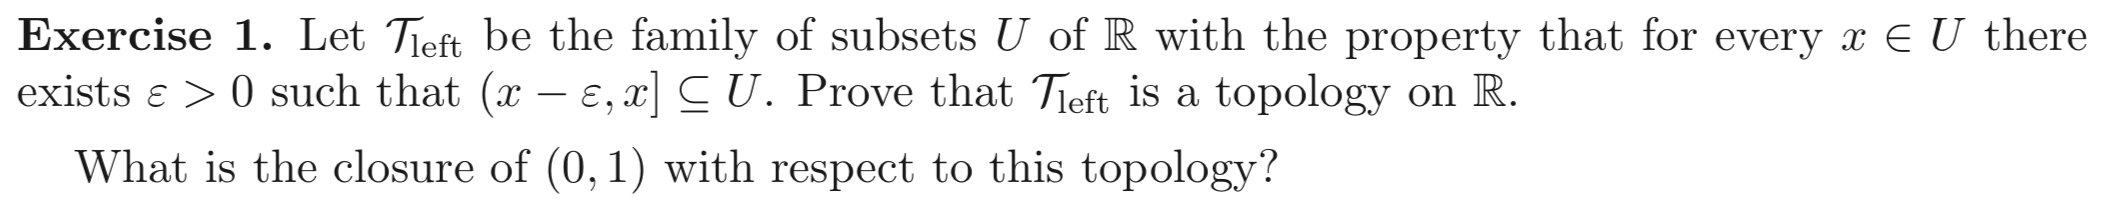
\includegraphics[width=400pt]{img/oxford-a5-1-1.png}
\end{mdframed}

\begin{proof}
  Let $\Tleft$ be the ``family'' of subsets $U$ of $\R$ such that for all $x \in U$ there exists
  $\epsilon > 0$ such that $(x - \epsilon, x] \subseteq U$.

  We must show that
  \begin{enumerate}
  \item $\Tleft$ is closed under finite intersections.

    Let $U_1, U_2 \in \Tleft$ and let $\epsilon_i:U_i \to \R^{>0}$ be such that
    $(x - \epsilon_i(x), x] \subseteq U_i$ for all $x$ in $U_i$, $i = 1, 2$.

    Let $x \in U_1 \cap U_2$ and let $\epsilon = \min(\epsilon_1(x), \epsilon_2(x))$.

    Note that the definition of $\epsilon_i$ implies that $(x - \epsilon, x] \subseteq U_1$ and
    $(x - \epsilon, x] \subseteq U_2$.

    Therefore $(x - \epsilon, x] \subseteq U_1 \cap U_2$, and so $U_1 \cap U_2 \in \Tleft$.

    Let $\bigcap_{i \in I} U_i$ be a finite intersection, where $I$ is a finite index set. Note
    that this intersection can be constructed by iterating the above argument, leading to the
    conclusion that $\bigcap_{i \in I} U_i \in \Tleft$ as required.

  \item $\Tleft$ is closed under arbitrary unions.

    We must show that $\bigcup_{i \in I} U_i \in \Tleft$ for any choice of index set $I$, whether
    finite, or countably infinite, or uncountably infinite.

    Suppose for a contradiction that there exists an index set $I$ such that
    $\bigcup_{i \in I} U_i \notin \Tleft$. Let $V = \bigcup_{i \in I} U_i$.

    Then there exists $x \in V$ such that for all $\epsilon > 0$ we have
    $(x - \epsilon, x] \not\subseteq V$.

    Note that $x \in U_i$ for some $i \in I$. Therefore there exists $\epsilon > 0$ such that
    $(x - \epsilon, x] \subseteq U_i$.

    But $U_i \subseteq V$, therefore $(x - \epsilon, x] \subseteq V$, a contradiction.
  \end{enumerate}
\end{proof}

\end{document}
